% l = 8
\begin{figure}[h]
\begin{center}
\subfloat{
\resizebox{8cm}{5cm}{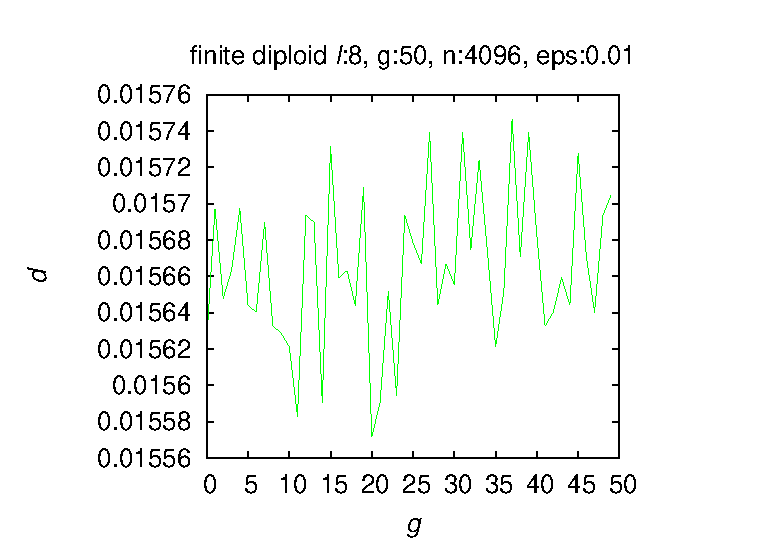
\includegraphics{figures/eps/vio/chi/b8/e0.01/n00004096_fin_dip.eps}}}\hspace{-3em}%
\subfloat{
\resizebox{8cm}{5cm}{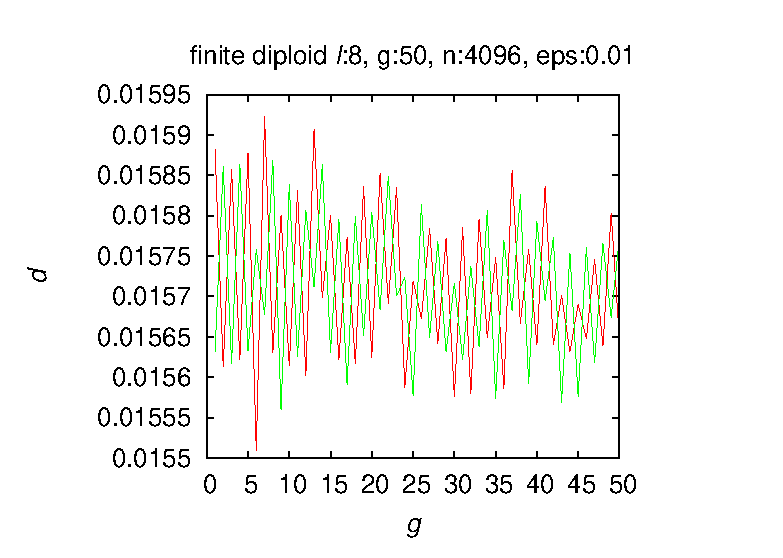
\includegraphics{figures/eps/vio/chi/b8/e0.01/n00004096_fin_dip_wovio.eps}}}\vspace{-1em}  \hspace{-3em}%
\end{center}
\begin{center}
\subfloat{
\resizebox{8cm}{5cm}{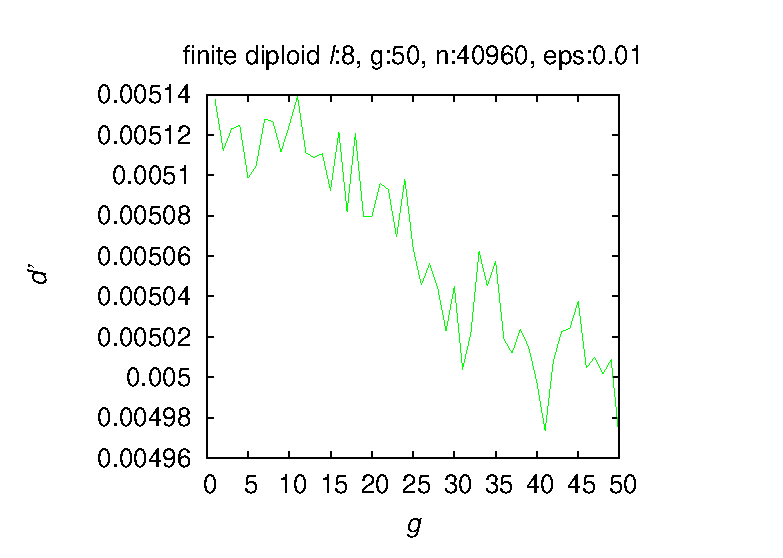
\includegraphics{figures/eps/vio/chi/b8/e0.01/n00040960_fin_dip.eps}}}\hspace{-3em}%
\subfloat{
\resizebox{8cm}{5cm}{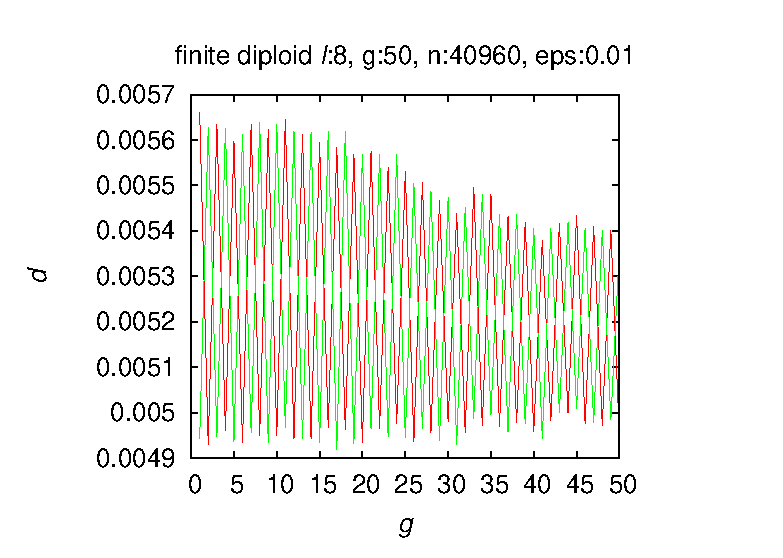
\includegraphics{figures/eps/vio/chi/b8/e0.01/n00040960_fin_dip_wovio.eps}}}\vspace{-1em}  \hspace{-3em}%
\end{center}


\begin{center}
\subfloat{
\resizebox{8cm}{5cm}{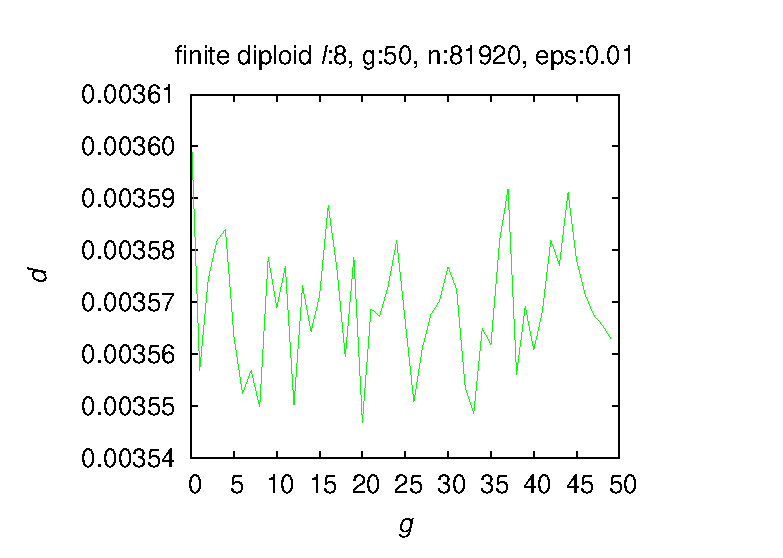
\includegraphics{figures/eps/vio/chi/b8/e0.01/n00081920_fin_dip.eps}}}\hspace{-3em}%
\subfloat{
\resizebox{8cm}{5cm}{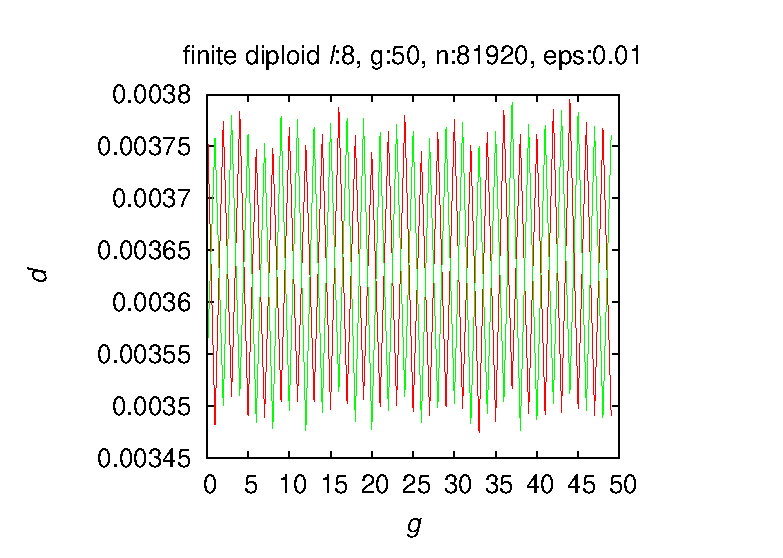
\includegraphics{figures/eps/vio/chi/b8/e0.01/n00081920_fin_dip_wovio.eps}}}\vspace{-1em}  \hspace{-3em}%
\end{center}

\begin{center}
\subfloat{
\resizebox{8cm}{5cm}{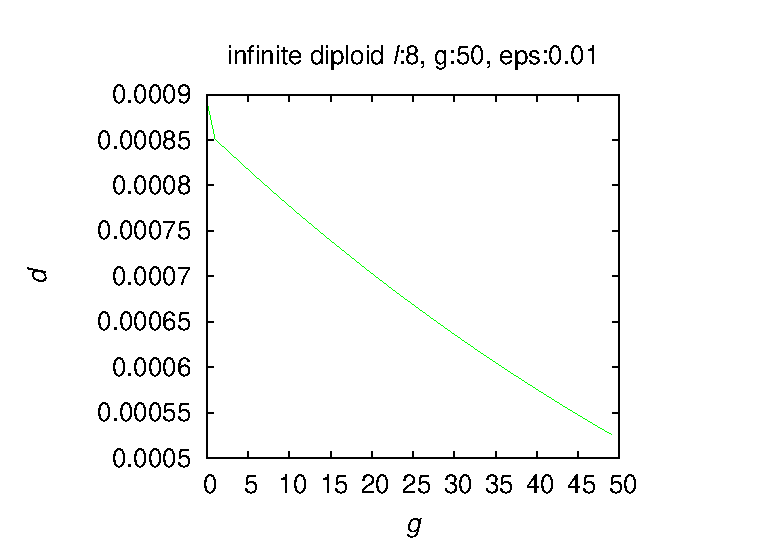
\includegraphics{figures/eps/vio/chi/b8/e0.01/inf_dip.eps}}}\hspace{-3em}%
\subfloat{
\resizebox{8cm}{5cm}{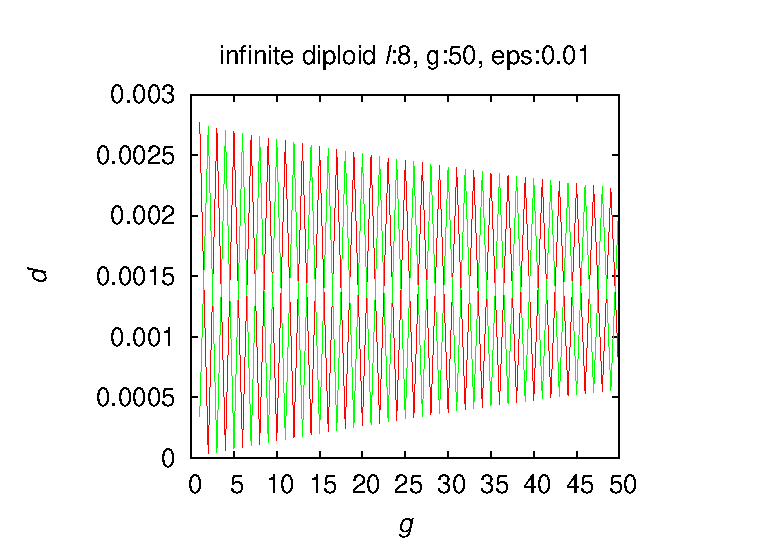
\includegraphics{figures/eps/vio/chi/b8/e0.01/inf_dip_wovio.eps}}}\vspace{-0.5em}  \hspace{-3em}%


\caption{\textbf{Infinite and finite diploid population oscillation behavior in case of violation in $\bm{\chi}$ for genome length $\ell = 8$ and $\bm{\epsilon} = 0.01$:} 
  In left column, $d'$ is distance of finite population of size $n$ or infinite population to limit $\bm{z}^\ast$ for $g$ generations. In right column, $d$ is distance of finite population or infinite population to limits $\bm{p}^\ast$ and $\bm{q}^\ast$ without violation.}
\label{oscillation_8d_vio_chi_0.01}
\end{center}
\end{figure}

% l = 10

\begin{figure}[h]
\begin{center}
\subfloat{
\resizebox{8cm}{5cm}{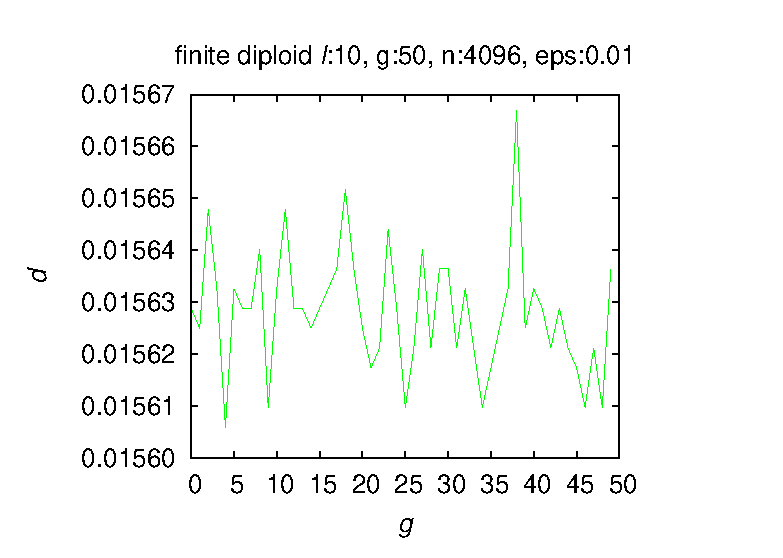
\includegraphics{figures/eps/vio/chi/b10/e0.01/n00004096_fin_dip.eps}}}\hspace{-3em}%
\subfloat{
\resizebox{8cm}{5cm}{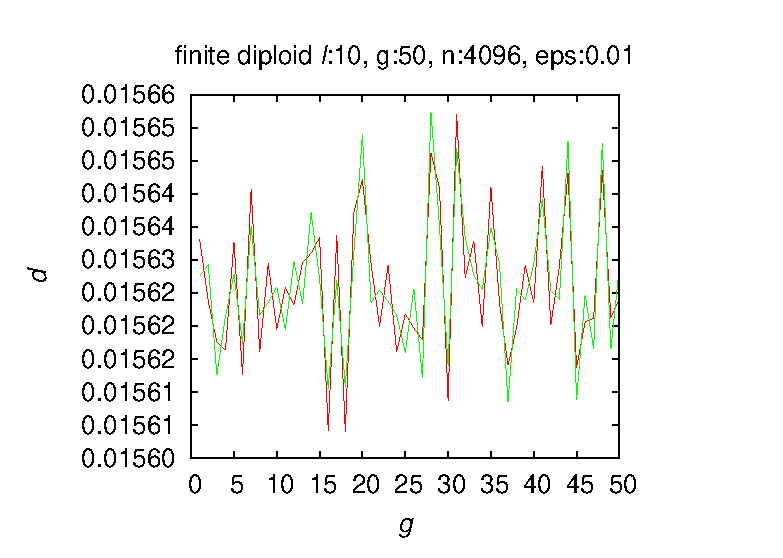
\includegraphics{figures/eps/vio/chi/b10/e0.01/n00004096_fin_dip_wovio.eps}}}\vspace{-1em}  \hspace{-3em}%
\end{center}
\begin{center}
\subfloat{
\resizebox{8cm}{5cm}{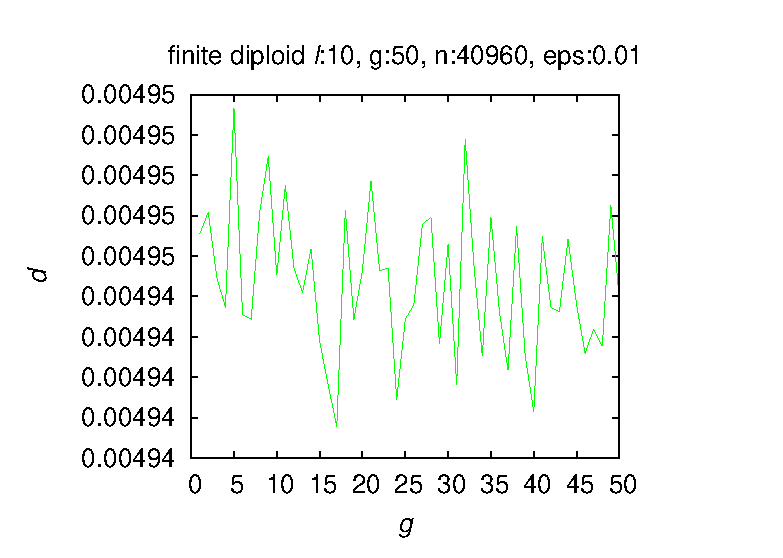
\includegraphics{figures/eps/vio/chi/b10/e0.01/n00040960_fin_dip.eps}}}\hspace{-3em}%
\subfloat{
\resizebox{8cm}{5cm}{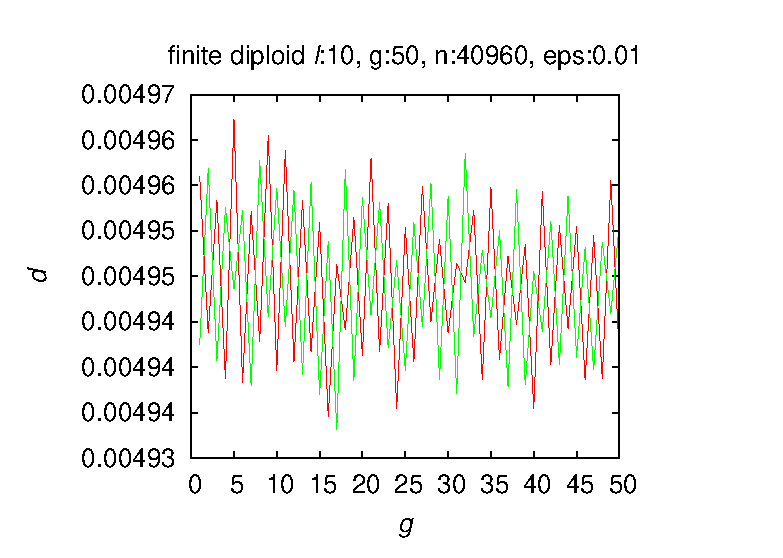
\includegraphics{figures/eps/vio/chi/b10/e0.01/n00040960_fin_dip_wovio.eps}}}\vspace{-1em}  \hspace{-3em}%
\end{center}


\begin{center}
\subfloat{
\resizebox{8cm}{5cm}{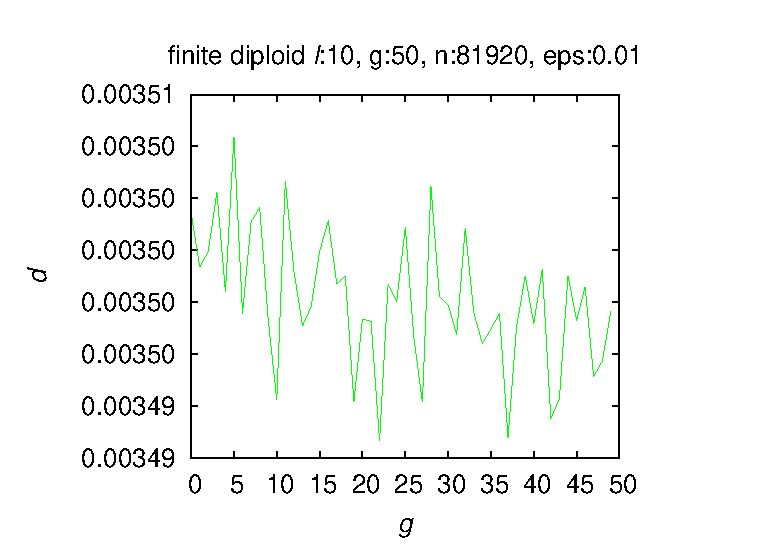
\includegraphics{figures/eps/vio/chi/b10/e0.01/n00081920_fin_dip.eps}}}\hspace{-3em}%
\subfloat{
\resizebox{8cm}{5cm}{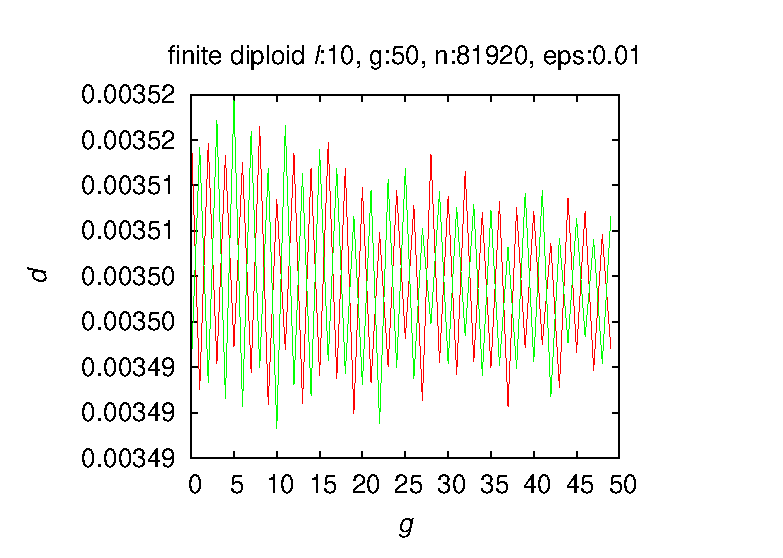
\includegraphics{figures/eps/vio/chi/b10/e0.01/n00081920_fin_dip_wovio.eps}}}\vspace{-1em}  \hspace{-3em}%
\end{center}

\begin{center}
\subfloat{
\resizebox{8cm}{5cm}{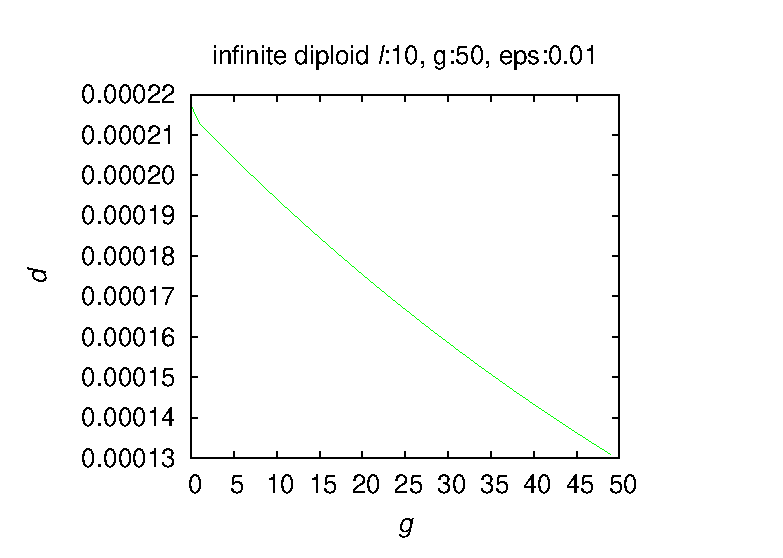
\includegraphics{figures/eps/vio/chi/b10/e0.01/inf_dip.eps}}}\hspace{-3em}%
\subfloat{
\resizebox{8cm}{5cm}{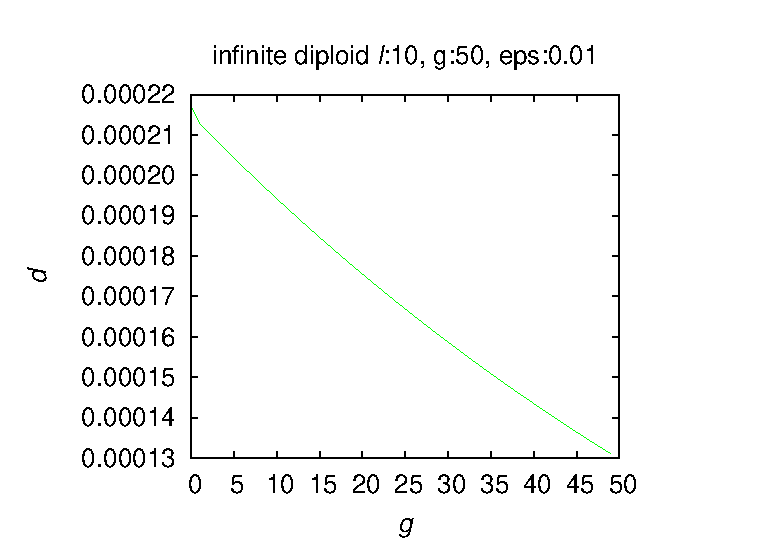
\includegraphics{figures/eps/vio/chi/b10/e0.01/inf_dip_wovio.eps}}}\vspace{-0.5em}  \hspace{-3em}%


\caption{\textbf{Infinite and finite diploid population oscillation behavior in case of violation in $\bm{\chi}$ for genome length $\ell = 10$ and $\bm{\epsilon} = 0.01$:} 
  In left column, $d'$ is distance of finite population of size $n$ or infinite population to limit $\bm{z}^\ast$ for $g$ generations. In right column, $d$ is distance of finite population or infinite population to limits $\bm{p}^\ast$ and $\bm{q}^\ast$ without violation.}
\label{oscillation_10d_vio_chi_0.01}
\end{center}
\end{figure}

% l = 12

\begin{figure}[h]
\begin{center}
\subfloat{
\resizebox{8cm}{5cm}{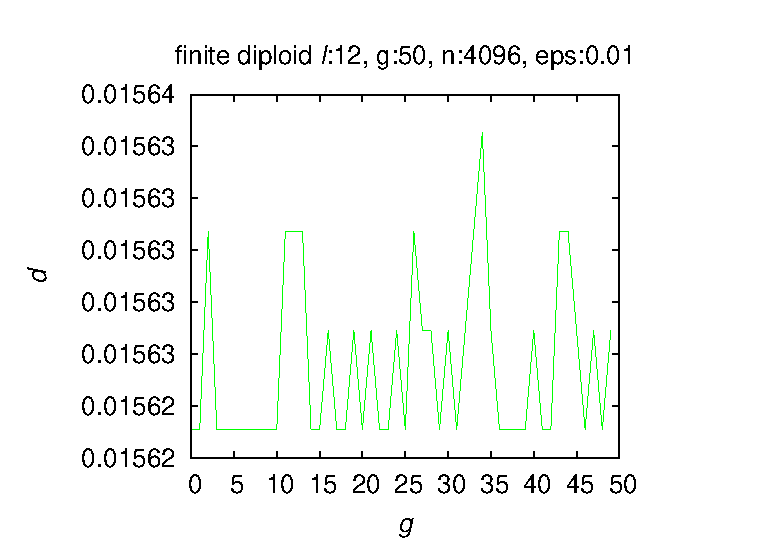
\includegraphics{figures/eps/vio/chi/b12/e0.01/n00004096_fin_dip.eps}}}\hspace{-3em}%
\subfloat{
\resizebox{8cm}{5cm}{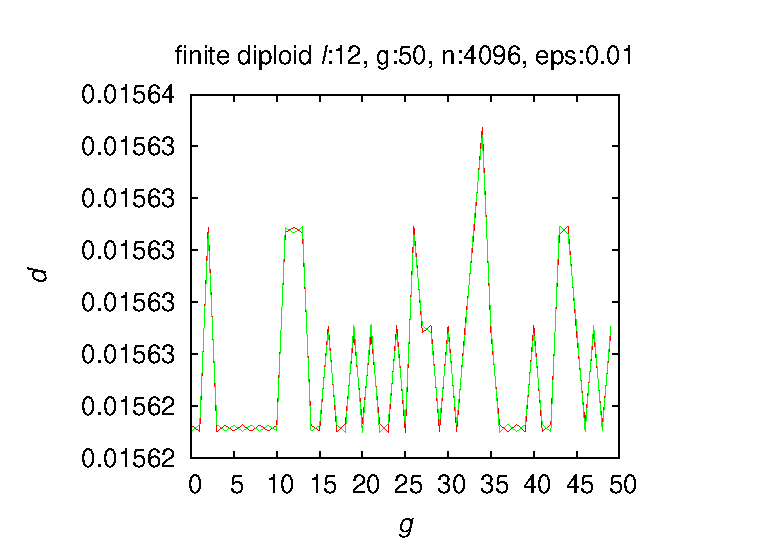
\includegraphics{figures/eps/vio/chi/b12/e0.01/n00004096_fin_dip_wovio.eps}}}\vspace{-1em}  \hspace{-3em}%
\end{center}
\begin{center}
\subfloat{
\resizebox{8cm}{5cm}{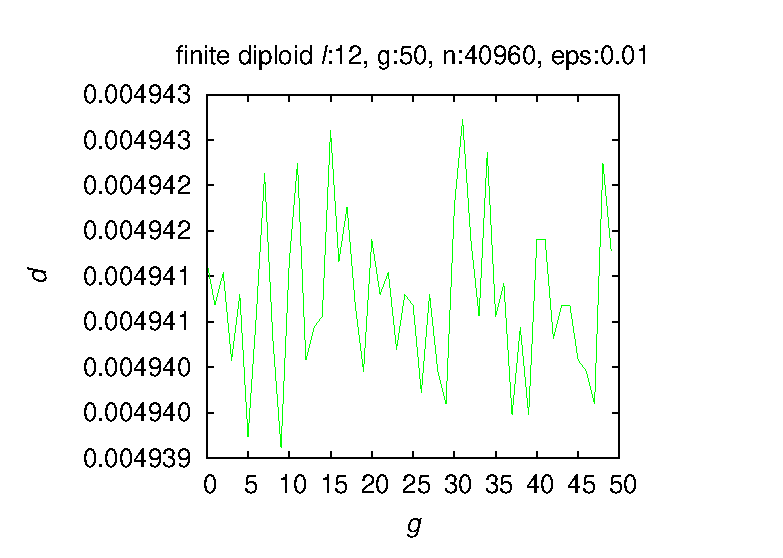
\includegraphics{figures/eps/vio/chi/b12/e0.01/n00040960_fin_dip.eps}}}\hspace{-3em}%
\subfloat{
\resizebox{8cm}{5cm}{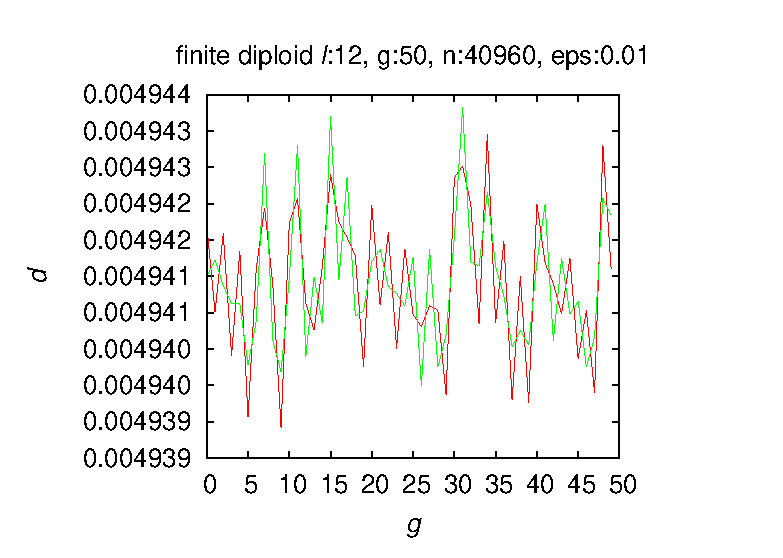
\includegraphics{figures/eps/vio/chi/b12/e0.01/n00040960_fin_dip_wovio.eps}}}\vspace{-1em}  \hspace{-3em}%
\end{center}


\begin{center}
\subfloat{
\resizebox{8cm}{5cm}{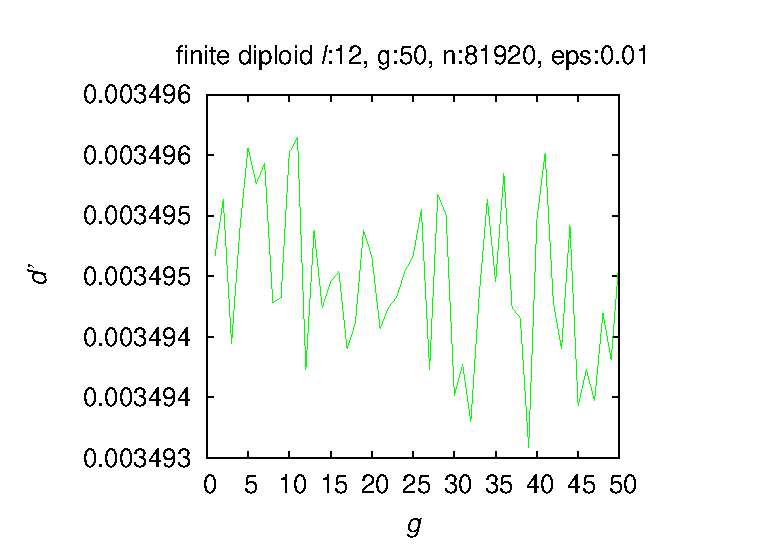
\includegraphics{figures/eps/vio/chi/b12/e0.01/n00081920_fin_dip.eps}}}\hspace{-3em}%
\subfloat{
\resizebox{8cm}{5cm}{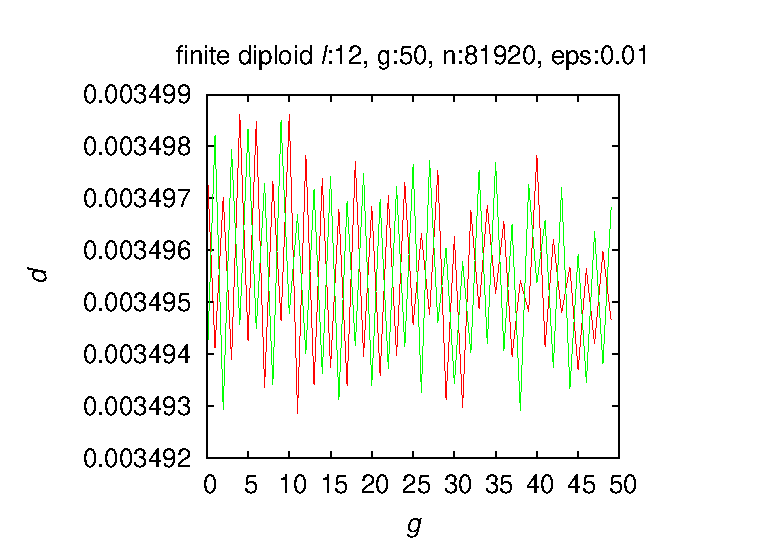
\includegraphics{figures/eps/vio/chi/b12/e0.01/n00081920_fin_dip_wovio.eps}}}\vspace{-1em}  \hspace{-3em}%
\end{center}

\begin{center}
\subfloat{
\resizebox{8cm}{5cm}{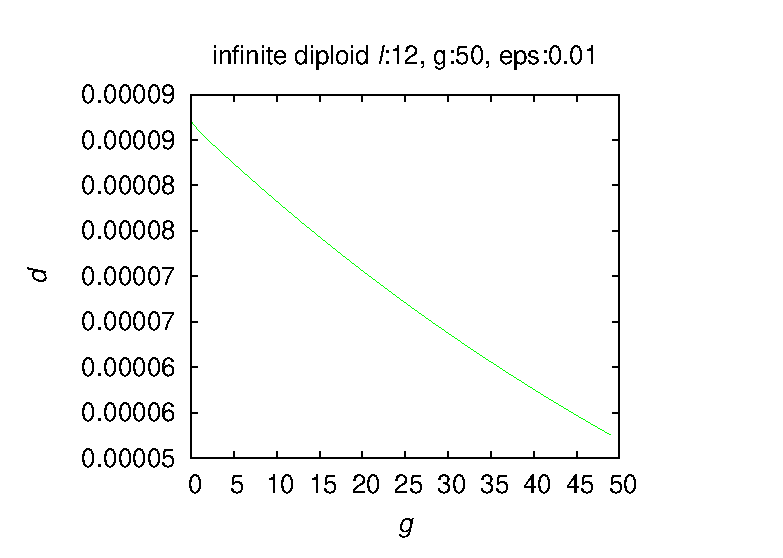
\includegraphics{figures/eps/vio/chi/b12/e0.01/inf_dip.eps}}}\hspace{-3em}%
\subfloat{
\resizebox{8cm}{5cm}{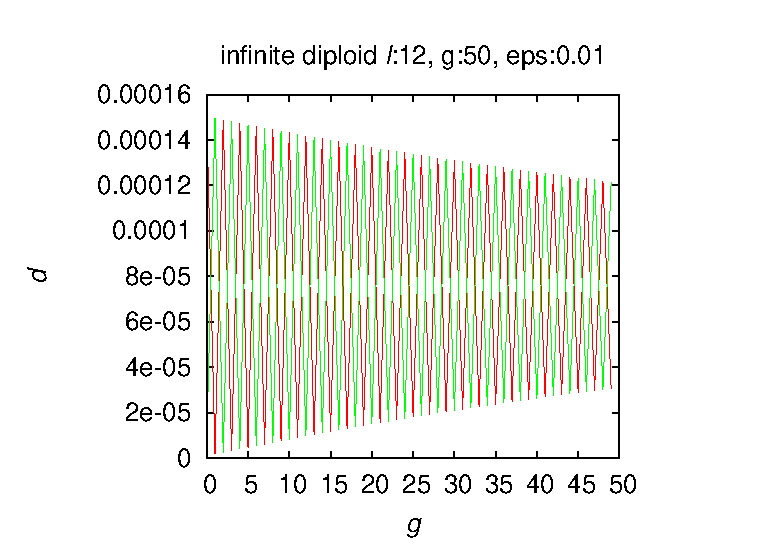
\includegraphics{figures/eps/vio/chi/b12/e0.01/inf_dip_wovio.eps}}}\vspace{-0.5em}  \hspace{-3em}%


\caption{\textbf{Infinite and finite diploid population oscillation behavior in case of violation in $\bm{\chi}$ for genome length $\ell = 12$ and $\bm{\epsilon} = 0.01$:} 
  In left column, $d'$ is distance of finite population of size $n$ or infinite population to limit $\bm{z}^\ast$ for $g$ generations. In right column, $d$ is distance of finite population or infinite population to limits $\bm{p}^\ast$ and $\bm{q}^\ast$ without violation.}
\label{oscillation_12d_vio_chi_0.01}
\end{center}
\end{figure}

% l = 14

\begin{figure}[h]
\begin{center}
\subfloat{
\resizebox{8cm}{5cm}{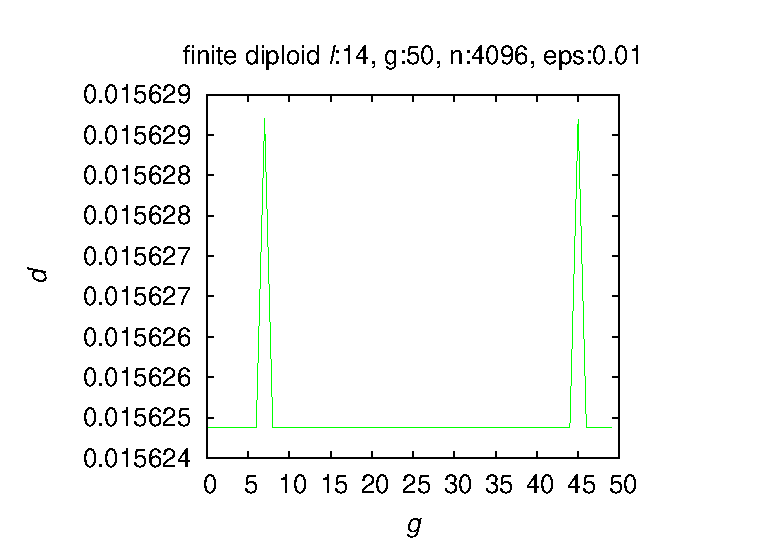
\includegraphics{figures/eps/vio/chi/b14/e0.01/n00004096_fin_dip.eps}}}\hspace{-3em}%
\subfloat{
\resizebox{8cm}{5cm}{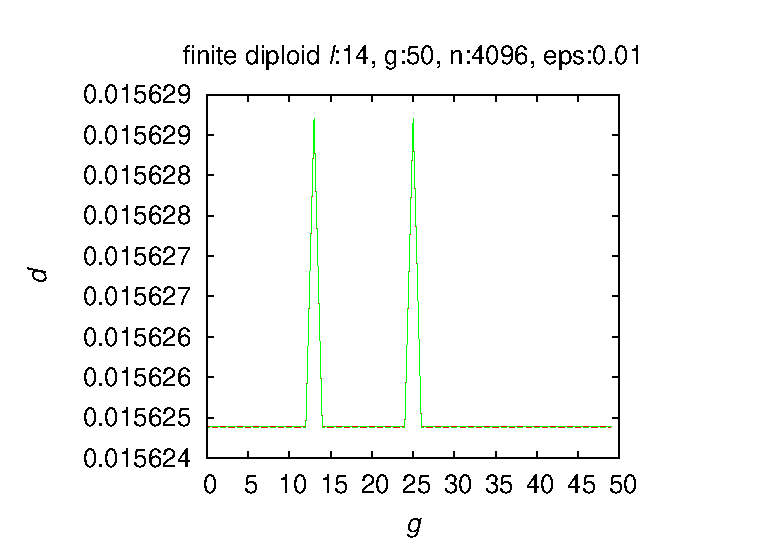
\includegraphics{figures/eps/vio/chi/b14/e0.01/n00004096_fin_dip_wovio.eps}}}\vspace{-1em}  \hspace{-3em}%
\end{center}
\begin{center}
\subfloat{
\resizebox{8cm}{5cm}{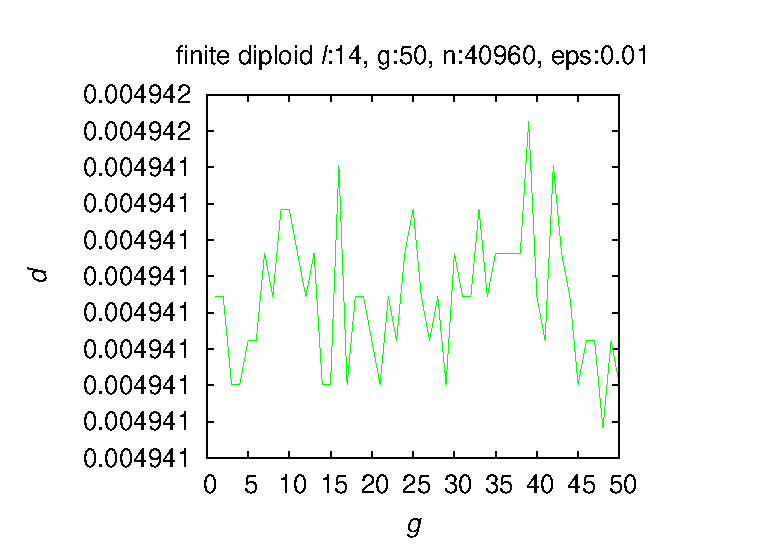
\includegraphics{figures/eps/vio/chi/b14/e0.01/n00040960_fin_dip.eps}}}\hspace{-3em}%
\subfloat{
\resizebox{8cm}{5cm}{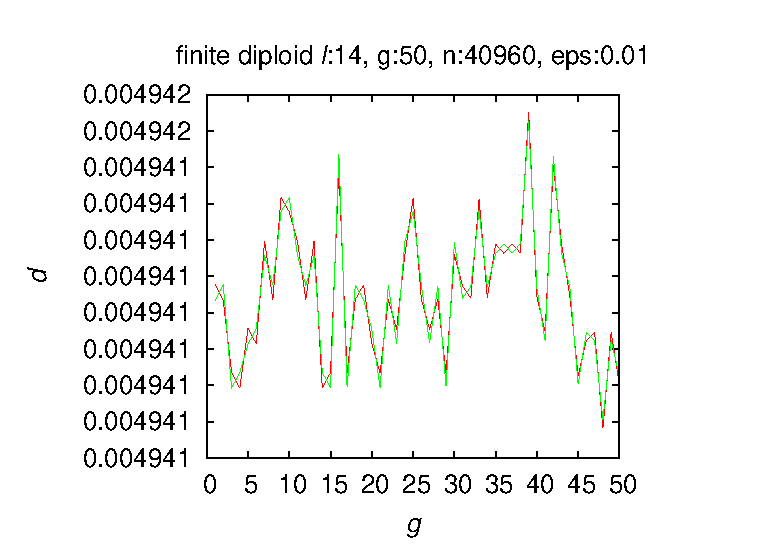
\includegraphics{figures/eps/vio/chi/b14/e0.01/n00040960_fin_dip_wovio.eps}}}\vspace{-1em}  \hspace{-3em}%
\end{center}


\begin{center}
\subfloat{
\resizebox{8cm}{5cm}{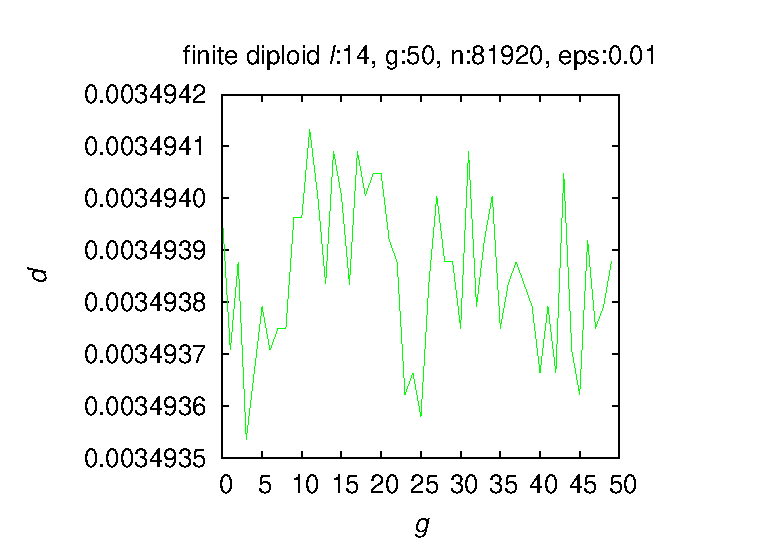
\includegraphics{figures/eps/vio/chi/b14/e0.01/n00081920_fin_dip.eps}}}\hspace{-3em}%
\subfloat{
\resizebox{8cm}{5cm}{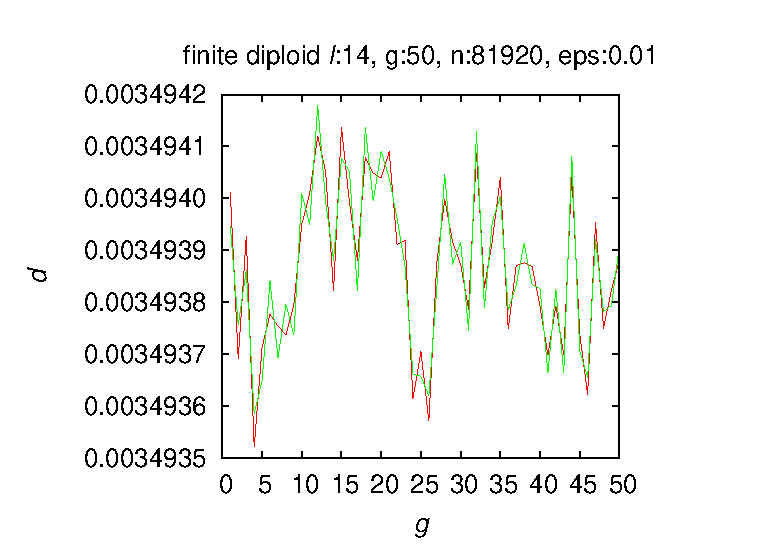
\includegraphics{figures/eps/vio/chi/b14/e0.01/n00081920_fin_dip_wovio.eps}}}\vspace{-1em}  \hspace{-3em}%
\end{center}

\begin{center}
\subfloat{
\resizebox{8cm}{5cm}{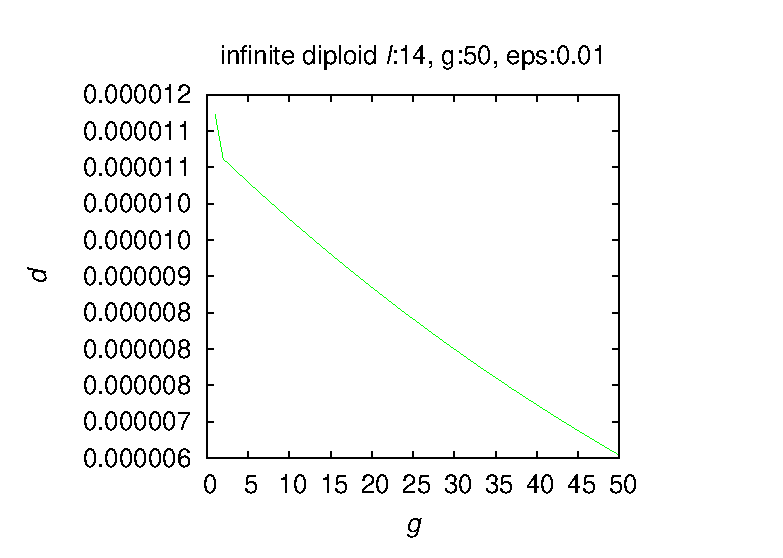
\includegraphics{figures/eps/vio/chi/b14/e0.01/inf_dip.eps}}}\hspace{-3em}%
\subfloat{
\resizebox{8cm}{5cm}{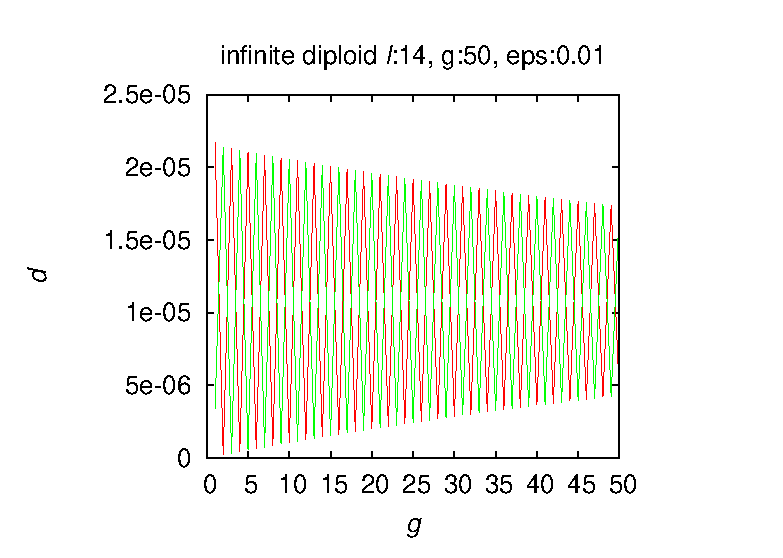
\includegraphics{figures/eps/vio/chi/b14/e0.01/inf_dip_wovio.eps}}}\vspace{-0.5em}  \hspace{-3em}%


\caption{\textbf{Infinite and finite diploid population oscillation behavior in case of violation in $\bm{\chi}$ for genome length $\ell = 14$ and $\bm{\epsilon} = 0.01$:} 
  In left column, $d'$ is distance of finite population of size $n$ or infinite population to limit $\bm{z}^\ast$ for $g$ generations. In right column, $d$ is distance of finite population or infinite population to limits $\bm{p}^\ast$ and $\bm{q}^\ast$ without violation.}
\label{oscillation_14d_vio_chi_0.01}
\end{center}
\end{figure}

\clearpage

The right column in figures \ref{oscillation_8d_vio_chi_0.01} through \ref{oscillation_14d_vio_chi_0.01} 
shows distance of finite and infinite diploid populations to non-violation limits $\bm{p^\ast}$ and $\bm{q^\ast}$ with $\bm{\epsilon} \;=\; 0.01$. 
Those graphs indicate oscillating behavior of diploid population given violation. 
Both finite and infinite populations oscillate given violation. Like in haploid case, oscillations are sharper. Since value of $\bm{\epsilon}$ 
is small, damping of ripples is slow. New masks created in crossover distribution with $\bm{\epsilon} \;=\; 0.01$ have small 
probability of being used during crossover. Infinite population oscillation does not die out completely in 50 generations. As value of $\ell$ 
increases, random drifting and wiggling of finite population occurs for small population size, and oscillation gets better with increase in population size. 
These are noticed more clearly in figures \ref{oscillation_12d_vio_chi_0.01} and \ref{oscillation_14d_vio_chi_0.01}.

The left column of figures \ref{oscillation_8d_vio_chi_0.01} through \ref{oscillation_14d_vio_chi_0.01} 
shows distance of finite and infinite diploid populations to limit $\bm{z^\ast}$ 
(limit with violation in crossover distribution $\bm{\chi}$) when $\bm{\epsilon} \;=\; 0.01$. 
The distance between finite population and limit $\bm{z}^\ast$ (limit with violation in $\bm{\chi}$ distribution) 
decreases as finite population size increases. 
The distance data for diploid population in case of violation in $\bm{\chi}$ distribution 
with $\bm{\epsilon} \;=\; 0.01$ for different finite population size $N$ are tabulated in table \ref{distanceChiDipEps0.01}.


\begin{table}[ht]
\caption{\textbf{Distance measured for violation in $\bm{\chi}$ with $\bm{\epsilon} \;=\; 0.01$ diploids:} $\ell$ is genome length, 
average distance between finite and infinite population is tabulated in the last three columns, and last row is expected single step distance.}
\centering
\begin{tabularx}{0.75\textwidth}{ c *{3}{X}}
\toprule
$\ell$ & $N = 4096$ & $N = 40960$ & $N = 81920$  \\
\midrule
8 & 0.0156	&  0.0051	& 0.0036 \\
10 & 0.0156	&  0.0049	& 0.0035 \\
12 & 0.0156	&  0.0049	& 0.0035 \\
14 & 0.0156	&  0.0049	& 0.0035 \\
\midrule
$1/\sqrt{N}$ & 0.0156 & 0.0049 & 0.0035 \\
\bottomrule
\end{tabularx}
\label{distanceChiDipEps0.01}
\end{table} 

From table \ref{distanceChiDipEps0.01}, average distance calculated for finite population size $4096$ is $0.0156$, 
for size $40960$ is $0.0050$ and for size $81920$ is $0.0035$. These results show average distance 
between finite population and limit $\bm{z^\ast}$ closely follows expected single step distance 
between finite and infinite population. The distance decreased as $1/\sqrt{N}$. 
Also, the distance is smaller in diploid populations than in haploid populations with $\bm{\epsilon} \;=\; 0.01$.


